\graphicspath{{images/}}
\section{Результаты моделей}
Так как данные очень хорошо линейно разделимы, явные выбросы были удалены, все модели дают одинаковый результат с поразительной точностью 98-88\%. 
Ниже приведены результаты всех моделей. Сначала модели, реализованные вручную, затем из библиотеки.

\subsection{Метод k-ближайших соседей}
\subsubsection{kNN}
\begin{alltt}
Best params: {'knn__k': 7}
Best acc: 0.9887333799860041
Accuracy: 0.9907640638119227
Recall: 0.994982438534872
Precision: 0.9885343968095713
\end{alltt}
\begin{center}
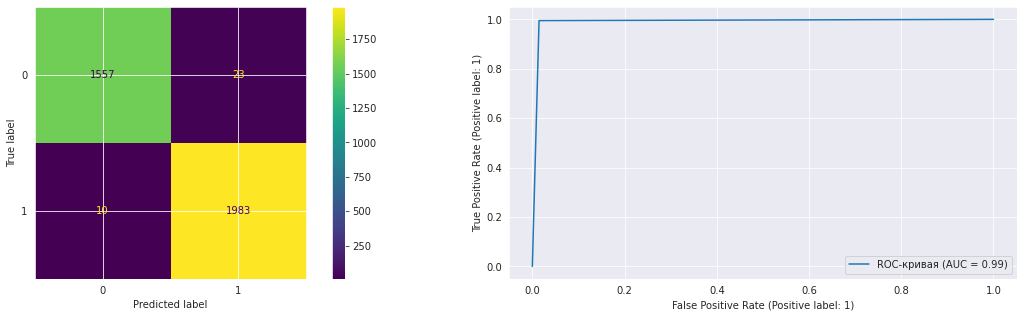
\includegraphics[width=\textwidth]{result_KNN}
\end{center}
\pagebreak

\subsubsection{sklearn.neighbors.KNeighborsClassifier}
\begin{alltt}
Best params: {'knn__n_neighbors': 7}
Best acc: 0.9887333799860041
Accuracy: 0.9907640638119227
Recall: 0.994982438534872
Precision: 0.9885343968095713
\end{alltt}
\begin{center}
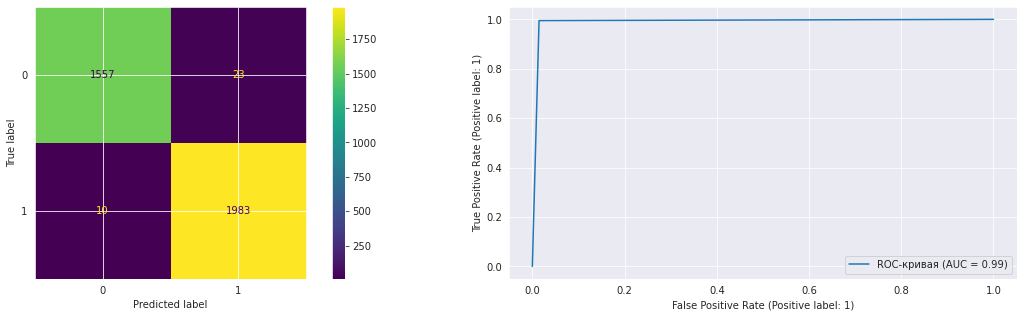
\includegraphics[width=\textwidth]{result_KNN_sc}
\end{center}
\pagebreak

\subsection{Логистическая регрессия}
\subsubsection{LogisticRegression}
\begin{alltt}
Best params: {'logreg__SGD_step': 0.1, 'logreg__batch_size': 5, 'logreg__epoches': 4}
Best acc: 0.9848845346396082
Accuracy: 0.9862860341449762
Recall: 0.9979929754139488
Precision: 0.9778761061946902
\end{alltt}
\begin{center}
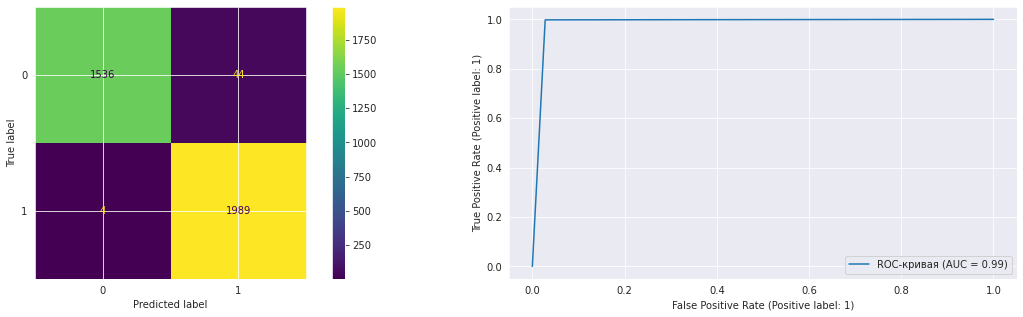
\includegraphics[width=\textwidth]{result_LR}
\end{center}

\subsubsection{sklearn.linear\_model.LogisticRegression}
\begin{alltt}
Best params: {'logreg__max_iter': 1000, 'logreg__penalty': 'none', 'logreg__solver': 'newton-cg'}
Best acc: 0.9898530440867738
Accuracy: 0.890848026868178
Recall: 1.0
Precision: 0.8363407469576164
\end{alltt}
\begin{center}
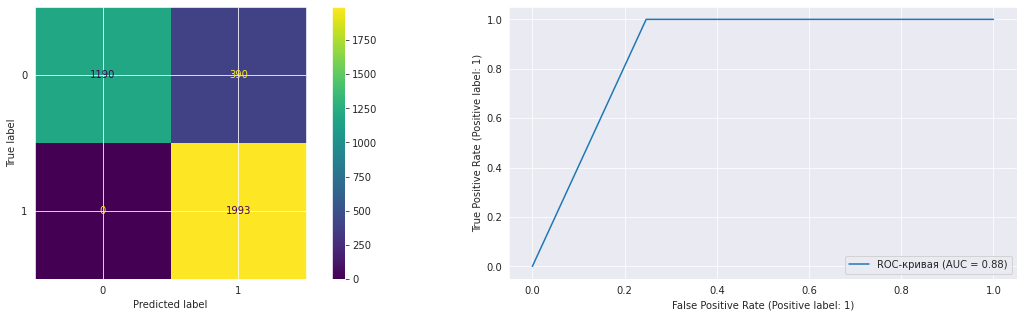
\includegraphics[width=\textwidth]{result_LR_sc}
\end{center}
\pagebreak

\subsection{Метод опорных векторов}
\subsubsection{SVM}
\begin{alltt}
Best params: {'SVM__SGD_step': 0.01, 'SVM__alpha': 0.1, 'SVM__batch_size': 20, 'SVM__epoches': 4}
Best acc: 0.979706088173548
Accuracy: 0.9851665267282396
Recall: 0.9979929754139488
Precision: 0.9759568204121688
\end{alltt}
\begin{center}
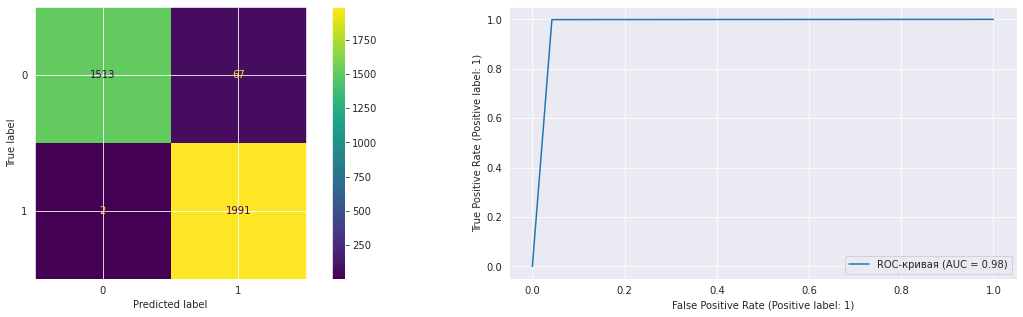
\includegraphics[width=\textwidth]{result_SVM}
\end{center}

\subsubsection{sklearn.svm.LinearSVC}
\begin{alltt}
Best params: {'svc__loss': 'squared_hinge', 'svc__max_iter': 100000.0}
Best acc: 0.987893631910427
Accuracy: 0.9888049258326337
Recall: 0.9954841946813848
Precision: 0.9846153846153847
\end{alltt}
\begin{center}
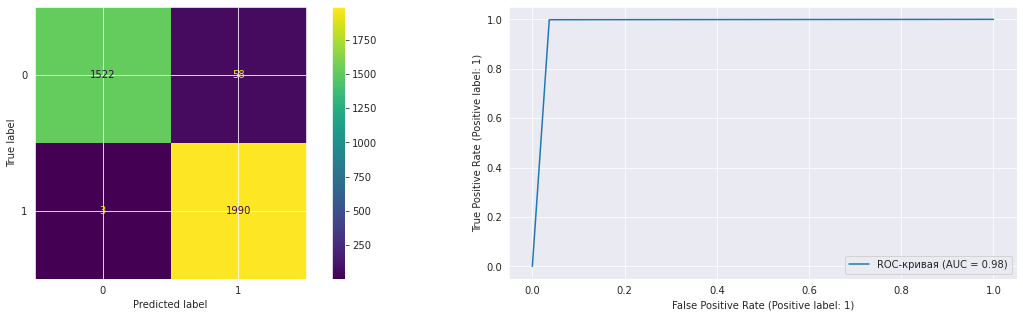
\includegraphics[width=\textwidth]{result_SVM_sc}
\end{center}
\pagebreak

\subsection{Наивный байесовский классификатор}
\subsubsection{NaiveBayes}
\begin{alltt}
Accuracy: 0.9860061572907921
Recall: 0.9959859508278976
Precision: 0.9792797237296498
\end{alltt}
\begin{center}
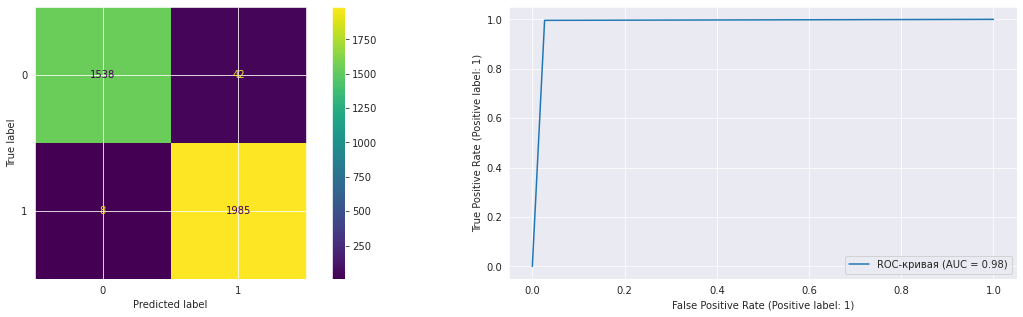
\includegraphics[width=\textwidth]{result_NB}
\end{center}

\subsubsection{sklearn.naive\_bayes.GaussianNB}
\begin{alltt}
Accuracy: 0.9851665267282396
Recall: 0.9984947315604616
Precision: 0.9754901960784313
\end{alltt}
\begin{center}
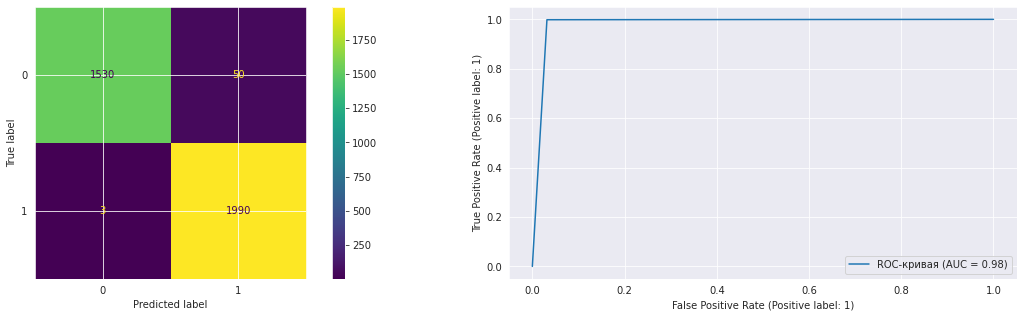
\includegraphics[width=\textwidth]{result_NB_sc}
\end{center}
\pagebreak

\subsection{Разделяющая прямая для метода опорных векторов}
\subsubsection{Моя реализация}
\begin{center}
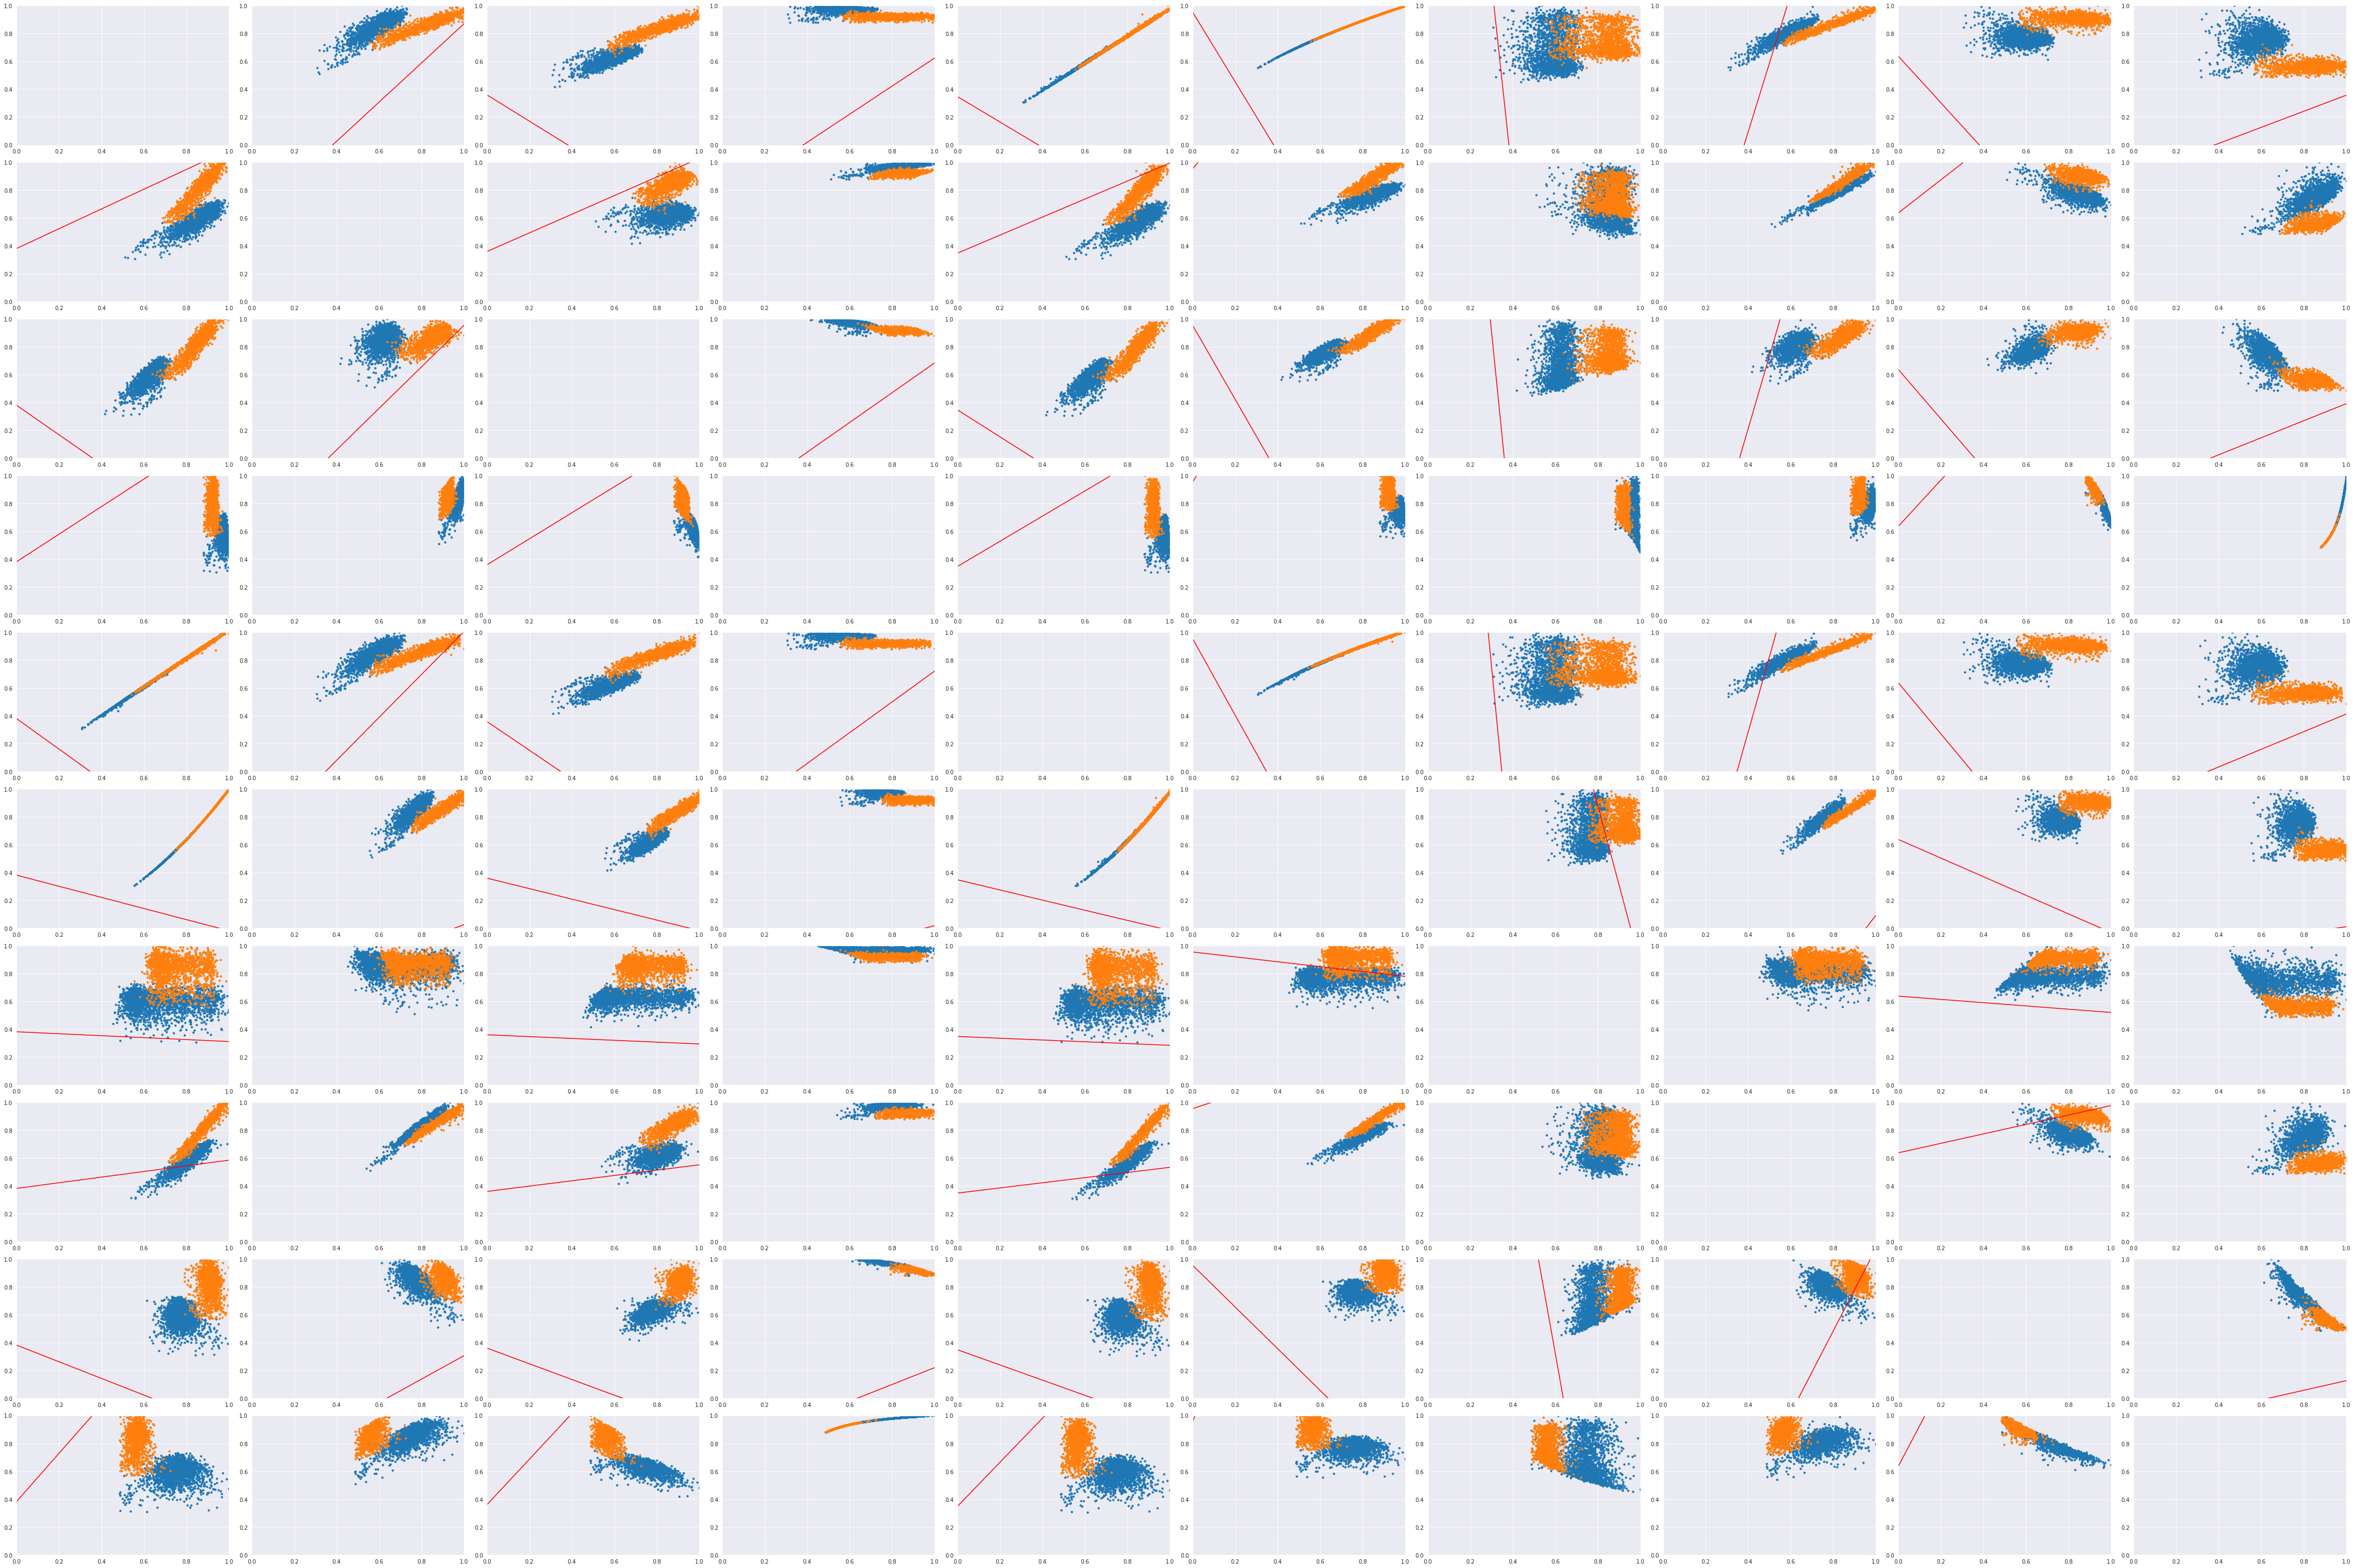
\includegraphics[width=\textwidth]{svm_lines_my}
\end{center}
\pagebreak

\subsubsection{sklearn.svm.LinearSVC}
\begin{center}
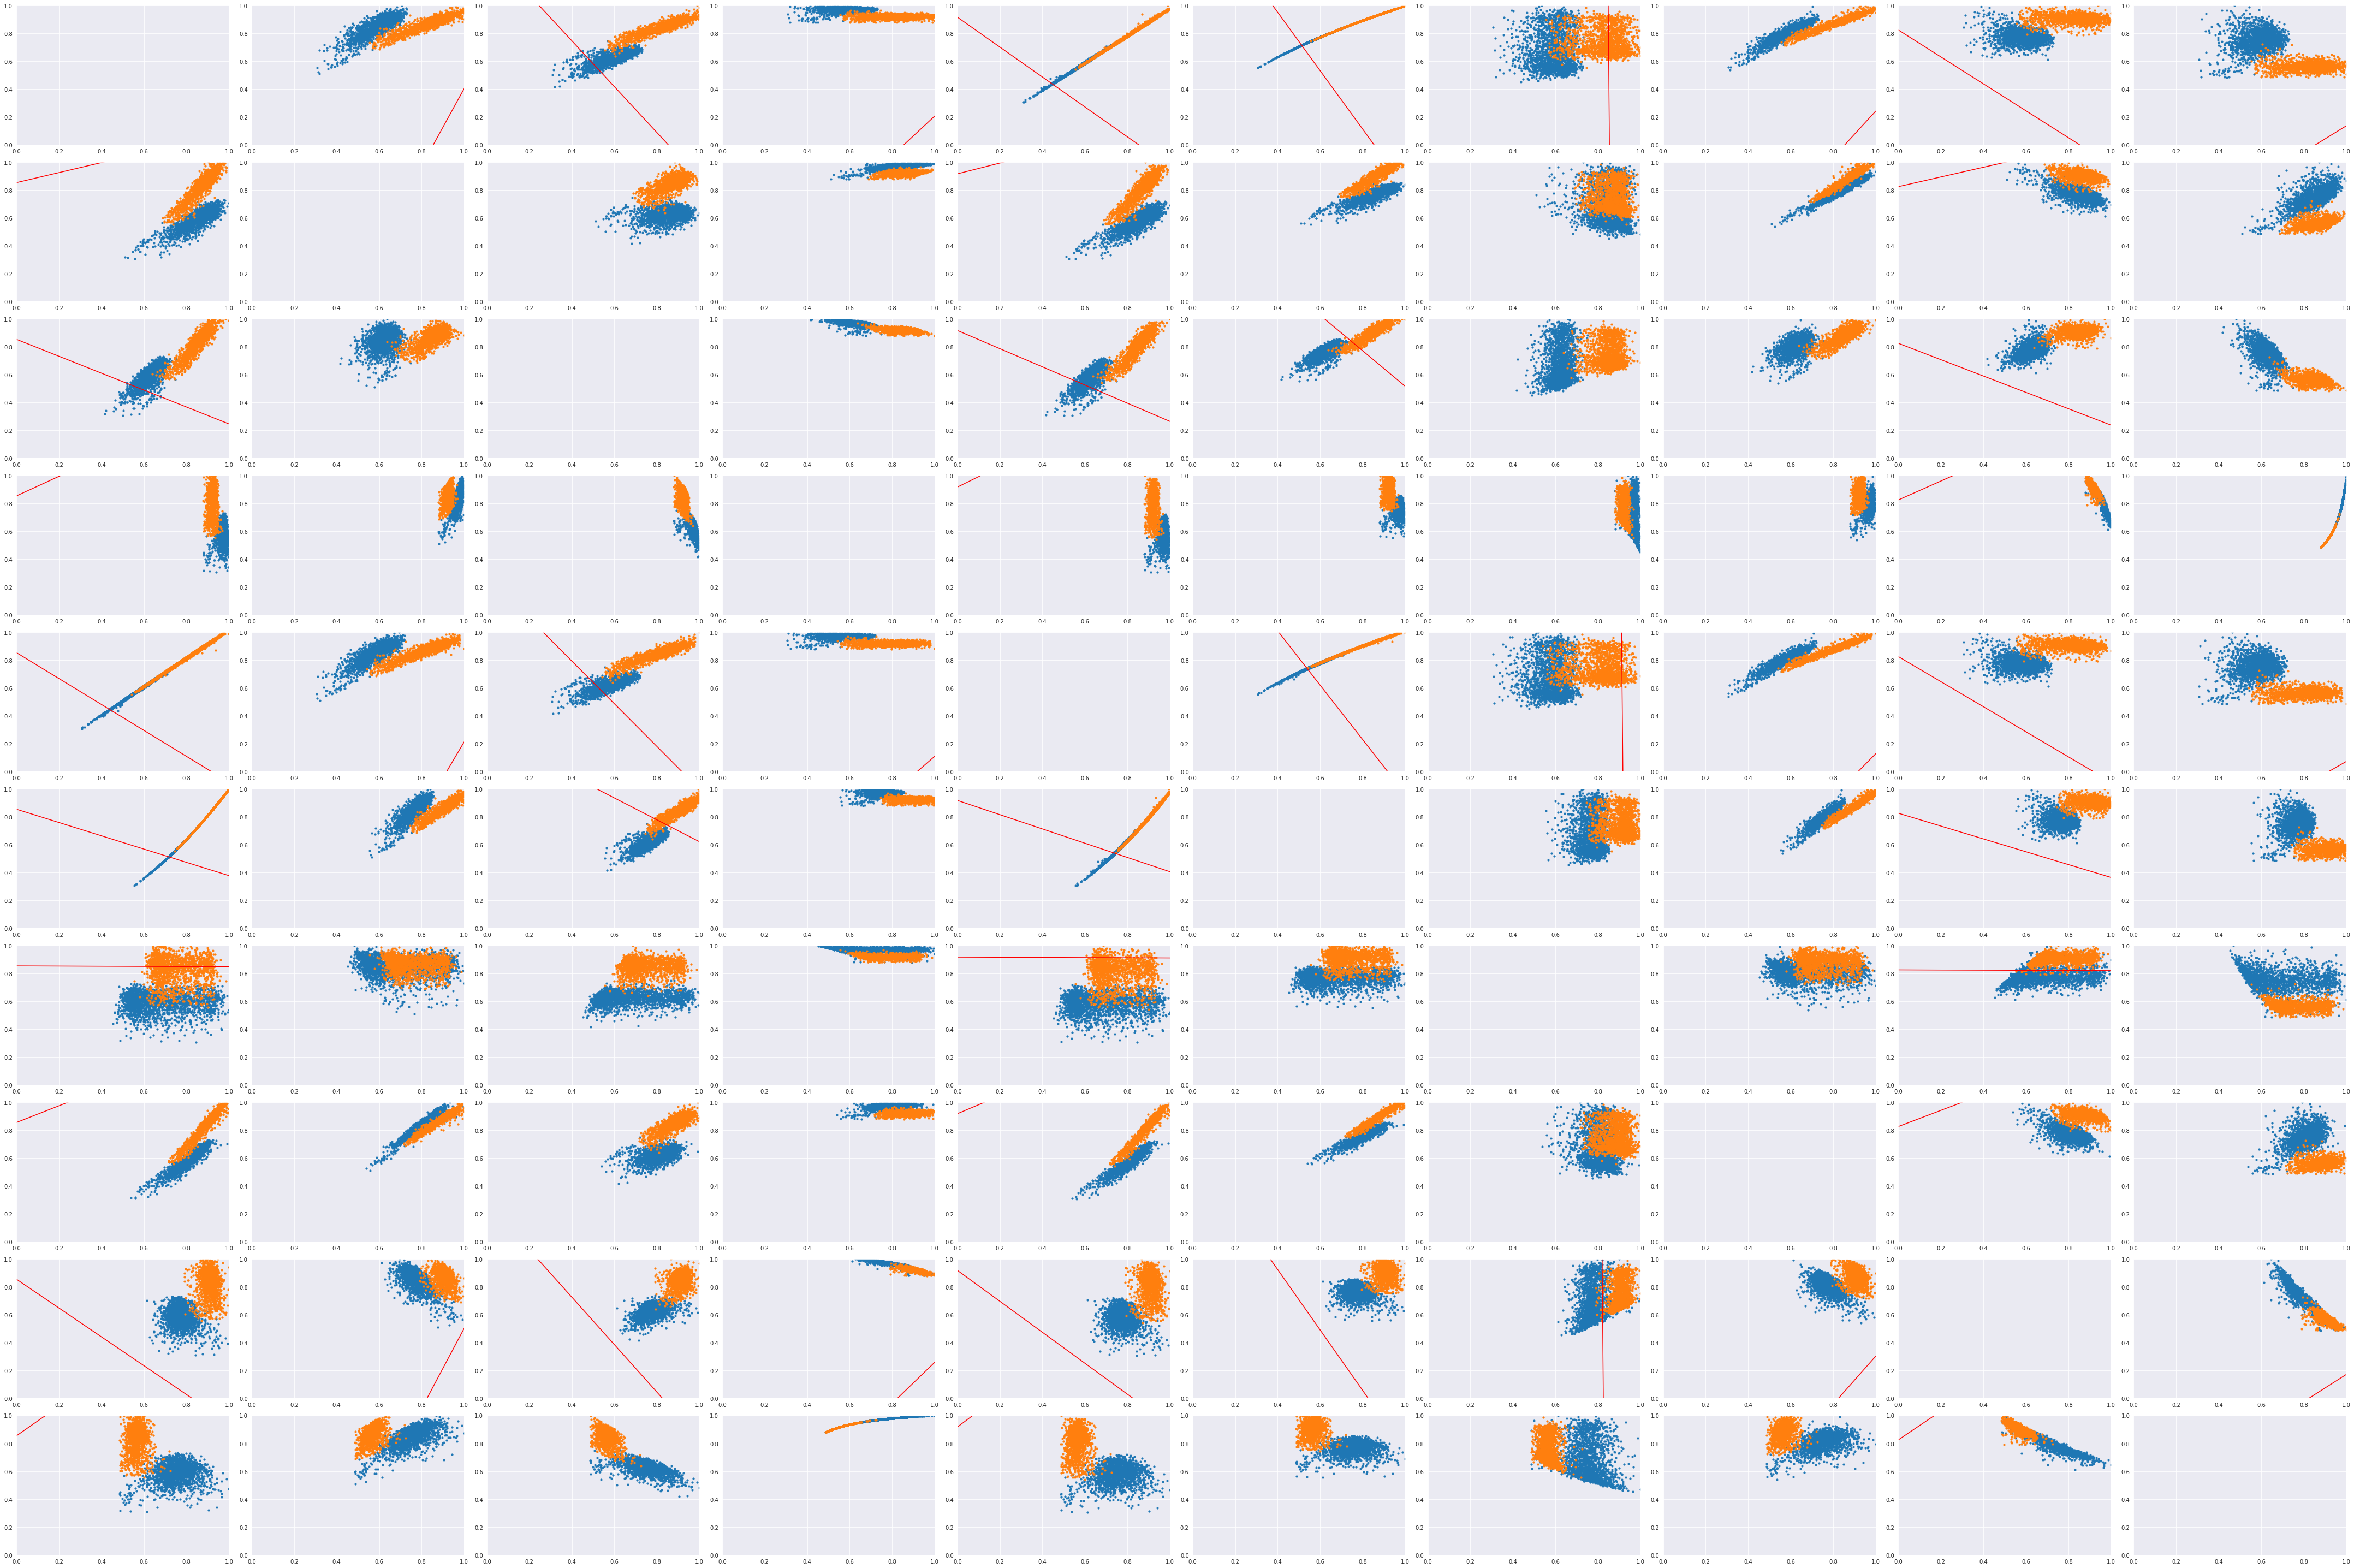
\includegraphics[width=\textwidth]{svm_lines}
\end{center}

\pagebreak
